%This chapter/section is about CC-inefficiency calculation 
%Created by kp on 9/15, 2013, with a copy of chap9moreCors/ccInefficiency.tex
%======= === Some notations ===========
%SEKpr==S. E. Kuhn's proof-reading;   SEKad = suggested additions by SEK
%============ =========================
\hspace{0.5cm}
% \newline \newline




%\newline  %double \newline gives underfull warnings
%\textbf{Elaborate more on the background contamination corrections.}

\section{Cerenkov Counter (CC) Efficiency}

In the EG4 experiment, the Cherenkov Counter (CC) signal plays a major part in forming the event trigger for %the CLAS detector and 
the data-acquisition system (DAQ). As stated earlier (see \ref{newCCsec}), for the purpose of achieving low \qsqs measurements with high detector efficiency\footnote{High detection efficiency is crucial for achieving smaller systematic uncertainties in the extracted physics quantities.}, a new %EG4 
dedicated CC was designed and placed in the sixth sector. Even though the new CC was designed to have a very high and uniform detection efficiency, some variation occurs over the covered kinematic range and therefore the knowledge of the detector efficiency as a function of the kinematics is required by our ``method of absolute cross-section difference''. %For example, if a significant amount of electrons are not detected by the CC, then the measured cross-section difference will be less than the actual value, thus affecting the extracted physics quantities accordigly. 
Therefore, a study was done to determine the CC efficiency as follows. 



\subsection{Procedure}

It is assumed that the efficiency for some specific kinematic bin depends on the average number of photoelectrons %(the corresponding variable in the data ntuple is ``nphe''), %SEKpr: Explain both trigger eff + nphe cut! 
produced by electrons in that bin which, in turn, is determined by the hit location on the Cerenkov PMT-projected plane %(defined by the projected \th and \ph) 
as well as the angle with which the %particle hit 
electron hits (or intersects) the plane. In the following, we describe how we determined the efficiency as a function of kinematic variables. %SEKadd: %SEKpr: Differentiate between AVERAGE (expected) nphe and (randomly distributed) measured nphe for one event


\begin{figure}[H] %ht, htpb (p - float, b = bottom, h=? t = top)
\centering
  %\leavevmode 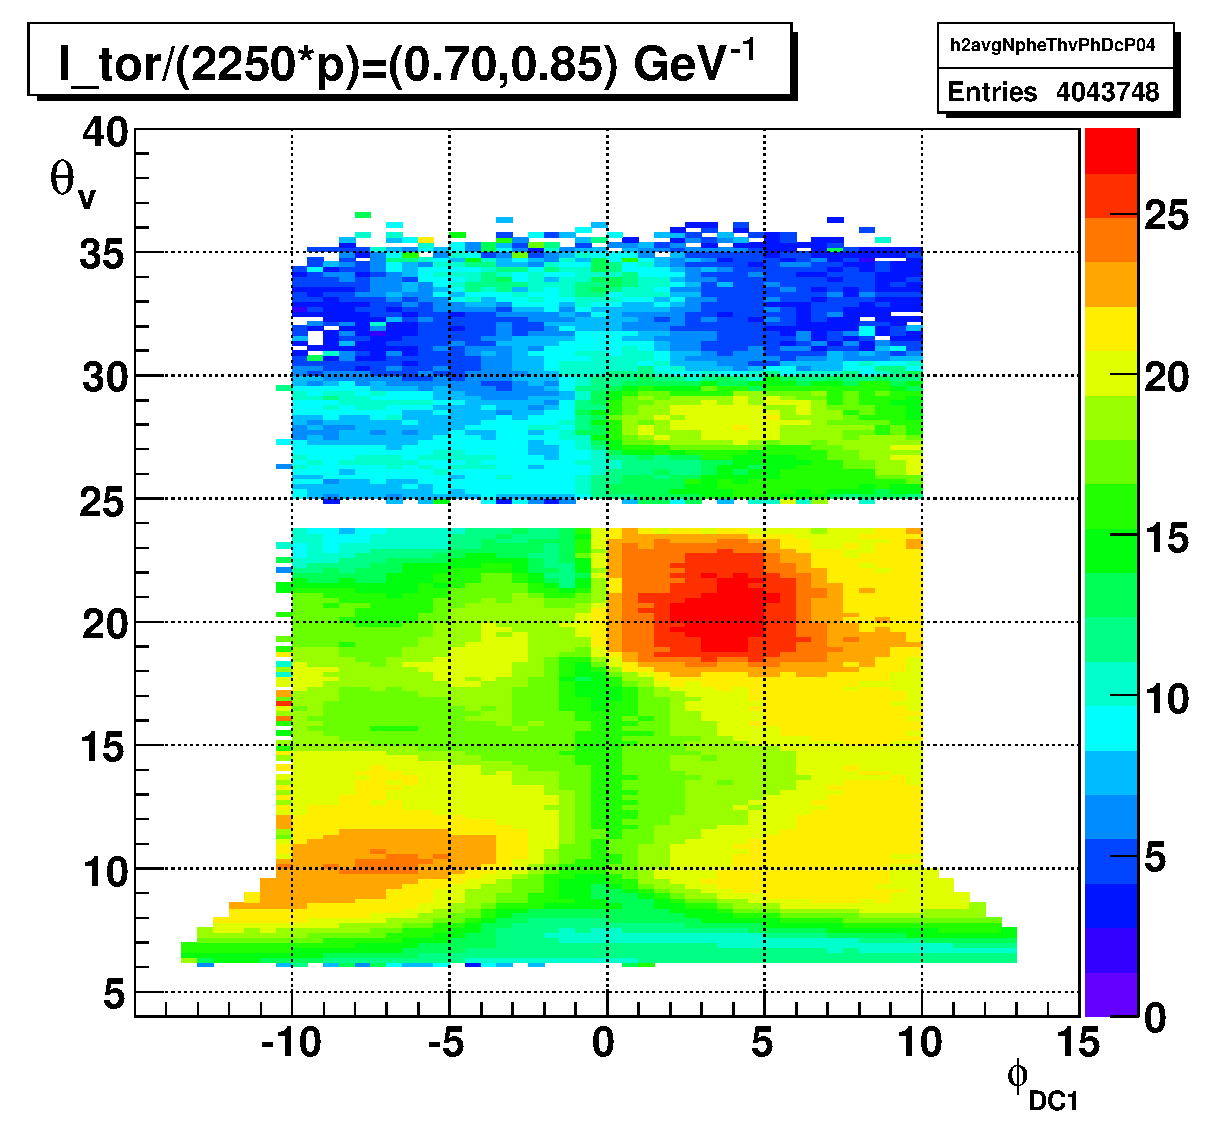
\includegraphics[width=0.9\textwidth]{chap4simul/FigConv/avgNpheFewBinEb3.eps} 
  \leavevmode 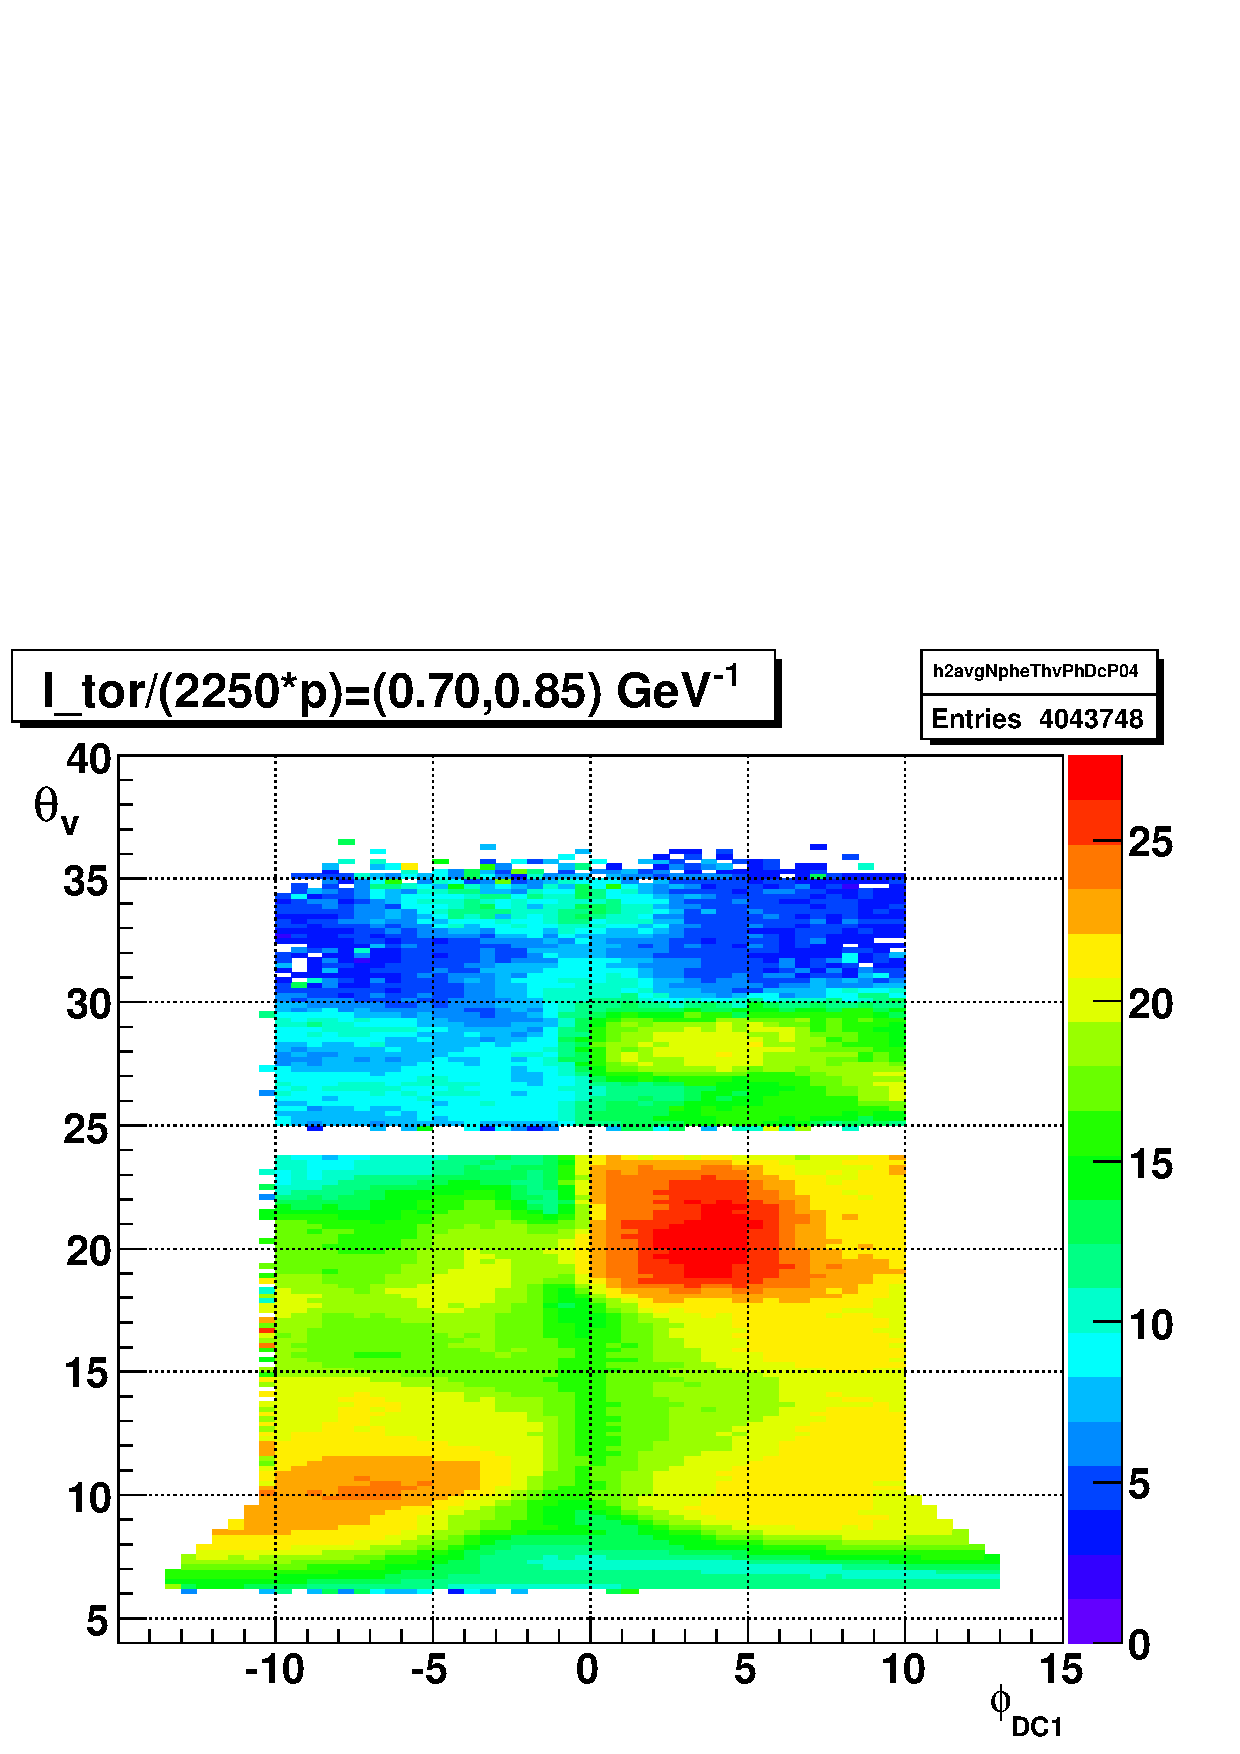
\includegraphics[width=0.9\textwidth]{TexmakerMyFinTh/chap4simul/FigConv/avgNpheFewBinEb3.png} 
  \caption[2D map of Nphe in a p-bin]{Average photoelectron number (color-coded) produced in the 6th sector CC as a function of $\theta_{vtx}$ and $\phi_{DC1}$ in the second bin of the variable $ip = (I_{tor}/2250)/p$ (from the 2.3 GeV \nh3 data).}
  \label{avgNpheEb3}
\end{figure}




%http://latex.mschroeder.net/index_en.php
\begin{enumerate}
\item First, we define a torus-current normalized inverse-momentum variable $ip = (I_{tor}/2250)/p$ (see above), and divide the whole 
kinematic space into 12 bins in ``ip'' as follows: (0.3, 0.4, 0.5, 0.6, 0.7, 0.85, 1.0, 1.25, 1.5, 1.75, 2.0, 2.25, 2.53). (For example, a 0.5 GeV electron during a 2 GeV run, which used 2250 A for torus current, would have ip = 2.0 GeV$^{-1}$) %SEKad: ip is proportional to the bend angle. (kp: bend due to mag. field?)
%\item Then, for each bin in ``ip'', average number of photoelectrons (Nphe) produced in the CC is mapped over the two dimensional phase space defined by the variables $\theta_{vtx}$ (scattering angle measured at the event vertex) and $\phi_{DC1}$ (azimuthal angle as measured at DC1). This map is made using data from proton production runs \footnote{This method relies on the use of a few "EC-only" type data runs that were collected without using CC in the trigger. Since this especial type of data were collected with proton as the  target, to be consistent, we chose to use proton production data to make the Nphe-maps.}, by using all the standard electron selection cuts except the Osipenko cuts.
\item Next, for each bin in ``ip'', a 2D map of the average number of photoelectrons %($N_{ph}$) 
is produced in a kinematic space defined by $\theta_{vtx}$ (scattering angle measured at the event vertex) and $\phi_{DC1}$ (azimuthal angle as measured at DC1). For this step, some data from NH$_3$ production runs\footnote{This method relies on the use of two different sets of data. One is the regular NH$_3$ target data and another is the ``EC-only'' %type
 data runs which were collected without using CC in the trigger. Since the latter type of data were collected with NH$_3$ as target, to be consistent, NH$_3$ production data was chosen rather than the ND$_3$ ones to make the $N_{ph}$-maps.} are used with the standard electron selection cuts. % (except the Osipenko cuts but requiring the condition that the electrons hit produced a signal in CC). %Since the Osipenko cuts are not used in this case, to ensure not many pions leaked into the electron sample, a very tight EC-cuts were develeped for this specific purpose and used 
%\footnote{To improve the purity of the electron samples, one may be tempted to use only elastic data for this purpose, but because we want CC-efficiency in all kinematics, using only elastic events is not a good idea.}. 
One of these average-nphe maps is shown in the Fig. \ref{avgNpheEb3}.  % SEKpr: such->these

%\textcolor{red}{Turns out, unlike what was written in ``thesisV1\_edited'', in the latest iteration of the work, I did use all the standard cuts (including osipenko in making the average nphe map. The earlier statement was a slip-up that sneaked in from the past writeup when I rushing to make the draft "ready".}

\item Next, using the ``EC-only-trigger'' %EC-trigger-only calibration 
data runs, %we choose  {elastic electron events} (to make sure they make the cleanest possible sample of electrons) that are expected to hit the central region of the CC, but using absolutely no actual CC information. %(Note that the CC-projected angles are used to decide whether the electrons hit the CC or not and these angles are calculated only from DC information, we do not, and should not use any actual CC information). 
good electron candidates are selected using the same cuts as before but without any CC-related cuts. %First of all, for 
For each of the selected electrons, the expected number of photoelectrons in the CC % it produces 
is determined in a look-up from %by looking at 
the above average $N_{ph}$-maps based on its momentum and angles. This expected $N_{ph}$ is then histogrammed in two ways - one histogram for those electrons which either didn't trigger CC or didn't pass all of the CC related cuts and another histogram for all %the
 electrons. The ratio of these two histograms (shown in the top-right and top-left panels of Fig. \ref{figccInefFits} respectively) gives us the inefficiency of the CC-detector as a function of $N_{ph}$ (as shown by the bottom two panels of the same figure). (Errors in the inefficiencies have not been drawn (for the purpose of cleaning) %cleanliness) 
 in the figures but they were calculated using the fact that the error in a ratio N2/N1 is $\sqrt{N2(1-N2/N1)}/N1$). %old formula that I used was $\sqrt{1/N2-1/N1}$ ). SEK says this seems wrong and he gave the following new formula: $$\sqrt{(N2/N1^2)(1-N2/N1)}$=\sqrt{N2(1-N2/N1)}/N1$

\item  The ideally expected CC intrinsic inefficiency is given by the %exp(-$N_{ph}$) 
Poisson distribution, since we require more than 2 photoelectrons, the theoretical prediction for the inefficiency is actually (1 + $N_{ph}$ + 1/2 $N_{ph}^2$)*exp(-$N_{ph}$). % in reality, it shows some discrepancy. To have a better analytical expression to represent the inefficiency we fit the data with a three parameter function of the form $y = p_0 + p_1 \cdot exp(-p_2 x)$, %SEKpr: Explain! again, mention cut + trigger!
However, we found empirically that if we calculate $N_{ph}$ only with electrons that exceed the threshold of 2.5, then we find that the functional form is pretty close to the form $y = p_0 + p_1 \cdot exp(-p_2 x)$, where x represents $<N_{ph}>$, and y represents the inefficiency. This form was used to fit with the above measured inefficiency and the result of the fit is shown in Fig.  \ref{figccInefFits}. We find that %kp: nearly agrees -> SEK: agrees very well
the inefficiency agrees very well with the expectation at low nphe, but remains at a very small constant value of around 0.01 (we call it the ``constant background'') at higher nphe. 

%\textcolor{blue}{You wrote in an email dated 11/3/13: Since we require more then 2 ph.els., the theoretical prediction for the inefficiency is actually $(1 + <nphe> + 1/2 <nphe>^2)exp(-<nphe>)$ - please correct our equation. However, we found empirically that if we calculate <nphe> only with electrons that EXCEED the threshold of 2.5, THEN we find that the functional form is pretty close to your y(x) form.}

%\textcolor{red}{Questen: How did you get $(1 + <nphe> + 1/2 <nphe>^2)*exp(-<nphe>))$? I am feeling even dumber these days}
%\textcolor{red}{SEK answer: From Poisson distribution: \\
%Probability for 0 phel = $ \frac{N^0}{0!}e^{-N} $ \\
%Probability for 1 phel = $ \frac{N^1}{1!}e^{-N} $ \\
%Probability for 2 phel = $ \frac{N^2}{2!}e^{-N} $ \\
%Probability for 2 or less phel = $ (1 + N + N^2/2) e^{-N} $ \\}


\begin{figure}[H] %[h] %ht, htpb (p - float, b = bottom, h=? t = top)
  \leavevmode 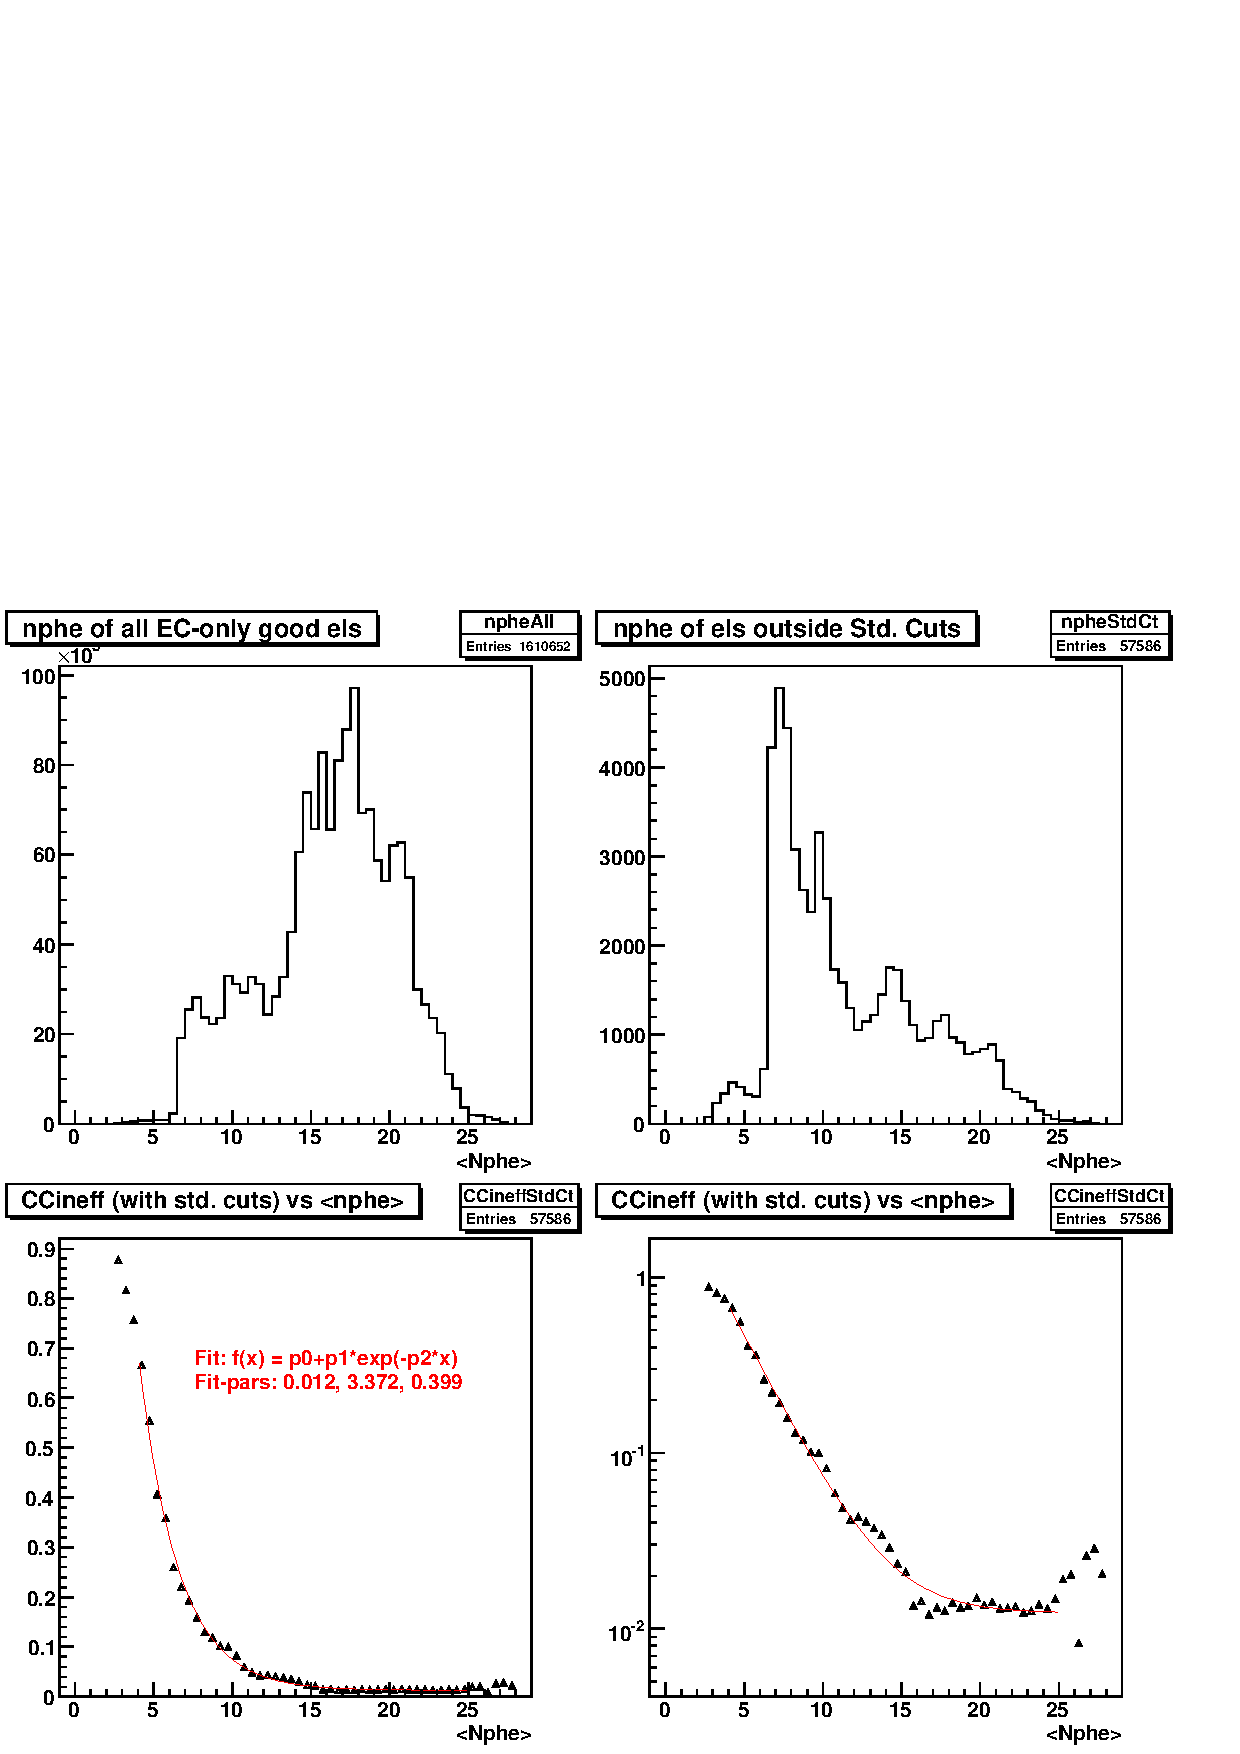
\includegraphics[width=1.0\textwidth]{TexmakerMyFinTh/chap4simul/FigConv/ccIneffPlotsEb3N.png} 
  \caption[Calculated CC-inefficiency]{EC detected good electrons (for all momenta) as a function of $<N_{ph}>$ (top left). Similar distribution (top right) for those good electrons that were detected by the EC but were rejected by the standard set of event selection cuts which includes CC-dependent cuts. By dividing the latter with the former, one gets the calculated CC inefficiency. The bottom two plots show the inefficiency distribution and a fit (red continuous line) in both linear (in third panel) and logarithmic (fourth panel) scales. Looking at the first plot, it can be seen that most electrons are above $N_{ph}=15$ where the inefficiency is at most 1-2 \%.}
  \label{figccInefFits}
\end{figure}

\item Finally we use the inefficiency fit just developed to evaluate the corresponding efficiencies and transform the 2D map of $N_{ph}$  into the corresponding efficiency maps (see Fig. \ref{ccEffMapEb3} for such a map in one momentum bin.). These maps are later used to apply the efficiency correction on an event by event basis in the simulation.
\end{enumerate}



\begin{figure}[H] %[h] %ht, htpb (p - float, b = bottom, h=? t = top)
  \leavevmode \includegraphics[width=1.0\textwidth]{TexmakerMyFinTh/chap4simul/FigConv/ccEffFewBinEb3.png} 
  \caption[CC-efficiency as a 2D map]{CC-efficiency in a momentum bin .}
  \label{ccEffMapEb3}
\end{figure}


%Since there were EC-only data available for only three beam energies (and also only on proton target), each of these three data sets were used to develop 3 different efficiency maps, which were then used in actual data analysis choosing one with the nearest beam energy. 
From this study, we see that the CC is very efficient in most of the kinematic region (see Fig. \ref{ccEffMapEb3}).
Once, the CC-(in)efficiency was estimated, we use the calculated CC efficiency to multiply our simulation (i.e., for each simulated event, we look up the CC efficiency and weigh the event with it. %The maximum effect of the systematic uncertainty in CC-inefficiency in the the measured physics quantities is estimated
%SEK: What do we do for systematic uncertainty on the inefficiency? (You mention it later, but it is always good to state it right away).









%===============================================================
% All the stuff below are all commented out
%\textbf{\textcolor{red}{Comment: This is old writeup, needs to be updated (along with the better/original resolution plots and new results) .}}\\ %\\%\newline
\begin{comment}
In the EG4 experiment, Cherenkov Counter (CC) signals provide a major part of the event triggers for the CLAS detector and 
the data-acquisition system (DAQ). To achieve very low \q2 values, the CLAS detector was run in the electron-outbending torus 
field configuration. In this case, the electron detection efficiencies (ratios of detected to incident numbers of electrons) of 
the standard CLAS Cerenkov Counters are strongly reduced and the performance over their coverage area become very non-uniform as 
well because they were designed for the inbending field configuration with different optics. Unlike the ``asymmetry method'' 
employed by the past high \q2 measurements which would have less/no dependence on the electron detection efficiency, we intend to 
measure the absolute cross-section difference to extract the structure functions and their moments because this method is assumed %kp: supposed 
to have smaller systematic uncertainties provided the detector inefficiencies are known or negligible. For that reason, an 
EG4-dedicated CC detector was designed and built by the INFN (Genova, Italy) collaborators which replaced the existing CC in the 
6th sector of CLAS. Even though, the new CC was designed to have a very high and uniform detection efficiency, %kp: that was not the case for our 
some variation occurs over our %SEK proof reading:  (5/14/5)
entire kinematic range and therefore the knowledge of the detector efficiency as a function of the kinematics %kp kinematic variable 
is required by our ``method of absolute cross-section difference''.
\end{comment}


\begin{comment}
\begin{figure}[htpb] %ht, htpb (p - float, b = bottom, h=? t = top)
  %\leavevmode \includegraphics[width=0.6\textwidth]{FigQualCheckBkGrnd/avgNpheAllEbProdRunsInvPbin1.eps} 
  \leavevmode \includegraphics[width=1.0\textwidth]{chap4simul/FigConv/ccIneffAvgNpheCropped.eps} 
  \caption{Average photoelectron number (color-coded) produced in the 6th sector CC as a function of projected \th and \ph in 
  the 2nd bin in variable $ip = (I_{tor}/2250)/p$.}
  \label{figavgNphe}
\end{figure}

\begin{figure}[htpb] %ht, htpb (p - float, b = bottom, h=? t = top)
  \leavevmode \includegraphics[width=1.0\textwidth]{chap4simul/FigConv/ccIneffIn2DCropped.eps} 
  \caption{Figure \ref{figavgNphe} converted to a 2D map of inefficiency using values from the fits as shown in \ref{figccInefFits}.}
  \label{figccInef2D}
\end{figure}


\begin{figure}[ht]
\centering
\subfigure[Y-axis in linear scale]{
\includegraphics[scale=0.36]{FigQualCheckBkGrnd/ccIneffGraphFitLinZ_elastEvs.eps}
\label{figccIneff1}
}
\subfigure[Y-axis in logarithmic scale]{
\includegraphics[scale=0.36]{FigQualCheckBkGrnd/ccIneffGraphFitLogZ_elastEvs.eps}
\label{figccIneff2}
}
%\caption[Optional caption for list of figures]{Caption of subfigures \subref{figsubfig1}, \subref{figsubfig2} and \subref{figsubfig3}}
\caption[]{CC-inefficiencies, the errors and the function obtained from the fit all plotted together against the number (nphe) of photoelectrons.}
\label{figccIneff} %Effect of Dc-smear
\end{figure}




\begin{figure}[htpb] %ht, htpb (p - float, b = bottom, h=? t = top)
  \leavevmode \includegraphics[width=1.0\textwidth]{FigQualCheckBkGrnd/fit2ccIneff.eps} 
  \caption{CC-inefficiency as a function of average-photo-electron number in linear (left) and logarithmic (right) scales.}
  \label{figccIneff}
\end{figure}
\end{comment}

\begin{comment} The cuts used are:
\begin{itemize} %Put a intra-thesis chapter/section link (rather than the web link) in thesis version
\item \href{http://www.jlab.org/Hall-B/secure/eg4/ripani/Reference/Reference.html}{groups 1, 2 and 4 cuts}. 
\item fiducial cuts
\item Eb-p[0] >= 0.0,   $\theta$>7.0,       15.0< $\theta_{proj}$ < 50.0, and  |$\phi_{proj}$| < 10.0
\item Electromagnetic Calorimeter (EC) cuts (Normal cut for elastic events, tight cut for inelastic/all events)
     % Normal EC cut: ECcut_el4ccIneff(Eb_index, p[0], ec_ei[cc[0]-1], ec_eo[cc[0]-1],  etot[cc[0]-1], beta); if(ecCut==false) return;
     % Tight  EC cut: if(etot[ec[0]-1]/p[0] <0.23  || etot[ec[0]-1]/p[0] < (-p[0]*0.29/5.0 + 0.29)) return;  //Just to get rid of the pions at low momenta 
\item Event is in sector 6 (such as using CC and EC sector cuts).
\item Requiring a hit in the CC, such as cc(ipart)$>$0. 
\item If elastic events used, |W - $M_{proton}$|< 0.1
\end{itemize}
\end{comment}
\begin{comment}
\item Using EC-trigger-only calibration runs, and applying the good electron cuts (listed below), one chooses good electron events 
(choosing only elastic electron events would be cleaner but that would limit statistics in many kinematic bins) that are expected 
to hit the central region of the CC, but using absolutely no actual CC information. Cuts to be used are:
\end{comment}
\begin{comment} Cuts used are:
\begin{itemize}
  \item group 1, 2 and 4 cuts;
  \item event is in sector 6 (such as using DC or EC sector cuts);
  \item must NOT require a hit in CC;
  \item a W cut to select elastically scattered electrons.
  \item fiducial cuts applied on projected theta and phi to select those events that are expected to hit the CC central region;
  \item EC-cuts to separate electrons from pions.
\end{itemize}
\end{comment}




\begin{comment}
\item  One can compare the result (\textbf{hist-5}) with the expected CC intrinsic in-efficiency which should be exp(-nphe). We find that 
hist \textbf{hist-5} agrees with this expectation at low nphe, but at high nphe remains at a very small constant value around 10E-3 (we call it the 
``constant background'').
\item Note on adding the hit angle (which is related to the momentum): One can simply repeat the whole procedure with different cuts 
on the momentum of the electron samples. One could have the difficulty that there are not so many elastic electron events for certain 
momentum bins for some \thp and \php bins.
\item     Note on cut efficiencies: One could study the CC intrinsic efficiency, just replace the cut of step 6 (requiring CC trigger) 
by the cut itself (such as nphe>### or any one of the Osipenko timing or geometrical matching cuts). Since I found the intrinsic distribution 
agrees well with Poison distribution, one could expect that the cut efficiency should also agree with Poison distribution. Doing step 11 
for the cut efficiency (but replacing exp(-nphe) by the proper function) could prove this.
\item     Note on runs/events to be selected: For intrinsic efficiency study one must use ``EC-trigger-only'' runs for step 4-11, alternatively 
one could use EC-only triggers (trigger bit 8) from all runs but it will be difficult to accumulate enough statistics. For other cut efficiency 
studies one can use ``regular" runs where CC is required in most of the triggers for steps 4-11, but keep in mind that the denominator of the 
efficiency analyzed this way are ``electron events that triggered CC", not ``all electron events". For regions where nphe is low the difference 
could be large due to low intrinsic efficiencies. 
\item How to use the efficiency results? The efficiency can be corrected on an event-to-event basis in the analysis using the 
expected nphe of the event: For intrinsic efficiency it follows the Poisson expectation at low nphe and the ``constant background'' 
at high nphe; For other cut efficiencies you replace these results by whatever you find.
\item Efficiencies were evaluated using four 1.3 GeV calibration runs (EC-trigger only, pass0). Elastic electrons were used. 
Both intrinsic efficiency and  efficiency of the Osipenko cut were extracted. %The program ``osicut_share.f'' in the directory shown above should give the efficiency results, as well as whether the event passes the Osipenko cuts whether it falls within the CC fiducial region.
\item Main reports on these cuts can be found on my weekly reports on 08/23/2007, 08/16/2007, and possibly a couple of weeks preceding them. 
\end{comment}
%\section{Pion Contamination Corrections}

%\section{\ep - Pair-symmetric Contamination Corrections}

